In this chapter, we describe the approach which we have adopted to create the dynamic benchmark of executable python software. The overall workflow of the approach is shown in the Figure \ref{fig:overall_approach}.

With the provided approach, our benchmark aims to achieve the properties of being large-scale, diverse, ready to run, ready to analyze, compositional and long term. We start with a large corpus of open source python projects listed in the awesome-python project (Section \ref{approach:corpus of python projects}). The projects are selected from this large corpus based on the selection criteria as described in Section \ref{approach:selection criteria}. This selection gives us a collection of python projects in the form of GitHub URLs and certain flags in a text file (Section \ref{approach:list of projects}). Bash scripts use this collection of projects in order to automate the installation of projects and their dependencies (Section \ref{approach:bash scripts}) which provides a set of installed python projects and the environment for use by developers and researchers as described in Section \ref{approach:collection of projects}. With the help of a python script (Section \ref{approach:python script}), a single command line interface provides easy access to the benchmark which consists of the installed projects along with various analysis tools and frameworks (Section \ref{approach:access interface}). The benchmark containing the installed projects along with its command line interface is packaged and exported as a docker container for use by researchers and developers (Section \ref{approach:packing and exporting}). The command line interface incorporates  analysis frameworks like LExecutor, DynaPyt and PyCG into the benchmark for execution of various tasks such as dynamic analysis, trace file generation, and static call graph generation respectively (Section \ref{approach:analysis framework}).

\begin{figure}[ht]
\centering
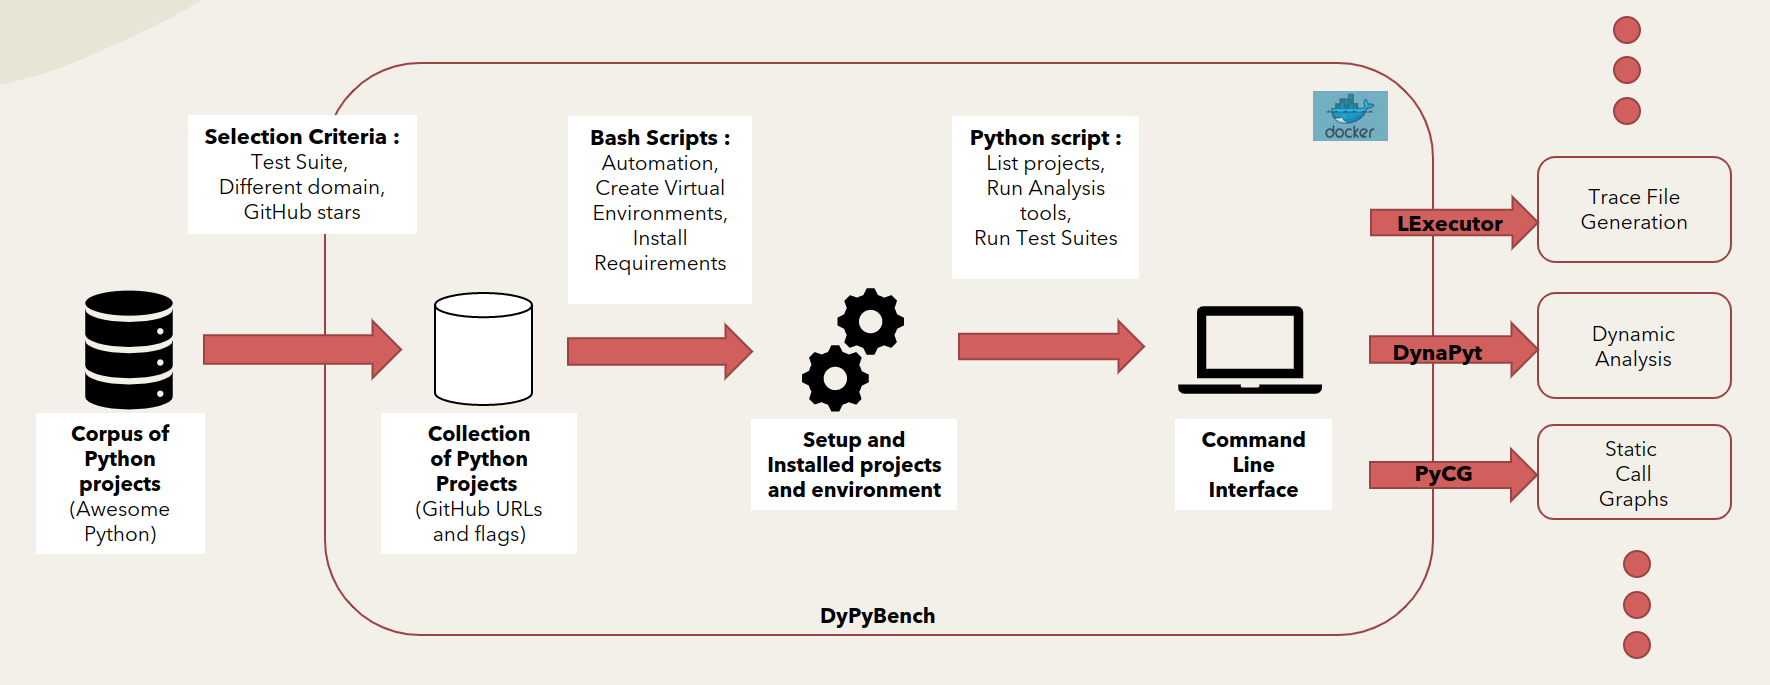
\includegraphics[width=1\linewidth]{figures/approach/DyPyBench.png}
\caption[Approach]{\label{fig:overall_approach}Overall Approach of DyPyBench.}
\end{figure}

\section{Corpus of Python projects}
\label{approach:corpus of python projects}
Python's ease of use and popularity, as well as the usage in different domains has led to a large number of projects being developed and made available to the community as open source software. GitHub alone contains more than 510000 public repositories that have python as their primary programming language \cite{bing_chat}(Bing Chat??). However, GitHub does not state which of these projects belong to which application domain. Also, it is difficult to go through 51000 repositories to filter out the projects from different domains without any classification.
This classification issue is solved with the help of Awesome-Python project, which is an open source project available on GitHub. This project contains a list of some of the most useful and interesting open source python projects including libraries, frameworks and software. Additionally, the awesome-python project classifies the python projects based on different categories which in essence represent the application domain of the project.
The awesome-python project acts as a corpus for our benchmark as it provides 679 python projects. It further classifies these projects into 92 main categories, out of which some of the categories can be further divided into sub-categories. Some of the categories and the number of projects in those are listed in table \ref{table:awesome-python}. For more details on the various categories and number of projects in each provided by the awesome-python project refer to the appendix \ref{appendix:awesome python projects}.

\begin{table}[ht]
    \centering
    \begin{tabular}{lc}
    \hline
    \textbf{Category} & \textbf{Number of Projects}\\
    \hline
    Admin Panels    & 9\\
    Code analysis   & 18\\
    Computer vision & 7\\
    Deep Learning   & 7\\
    Documentation   & 3\\
    Files   & 7\\
    GUI development & 16\\
    Robotics    & 2\\
    Task Queues & 5\\
    Web Frameworks  & 5\\
    \hline
    \end{tabular}
    \caption{Project Categories (Awesome Python)}
    \label{table:awesome-python}
\end{table}

\section{Selection Criteria}
\label{approach:selection criteria}
The corpus of python projects provides us with a large number of python projects to choose from diverse application domains. However, the benchmark must contain a restricted number of projects which fulfill the requirements that can make benchmark useful for its intended purpose. The selection criteria does exactly this for our benchmark, i.e., it makes our benchmark large scale and diverse by selecting 50 python projects from the available corpus. The selection criteria of diverse domain ensures that we select the projects which belong to different categories as described in the section \ref{approach:corpus of python projects}. The count of 50 projects ensures that we have sufficiently large number of projects in the benchmark for usage by different analysis tools. Since, in this work we are creating a dynamic benchmark we focus on the projects for which we can perform execution. Test suites provide us with a files which can be easily execute the code using testing libraries such as pytest, unittest, flake8, etc. As a result we include the criterion of presence of test suites for the selection process. However, we limit the execution of tests via pytest as it is a popular testing library and is also used by the DynaPyt framework used for analysis. The number of stars a project has on GitHub is be an indication of how popular and well-regarded it is in the community. More stars generally mean more people have found the project useful and interesting, and it has a larger user base and community of contributors. Since a benchmark must contain useful and meaningful projects, we include the criterion of a minimum 500 GitHub stars for the project selection. This is also a common practice among benchmarks in other languages such as Java Microbenchmark Harness (JMH), and Google Benchmark. 

\section{List of Python Projects}
\label{approach:list of projects}
Applying the selection criteria as described in section \ref{approach:selection criteria} we obtain a list of 50 open-source python projects from diverse application domains. Since, the projects have their own installation dependencies and source code structure, we need a generic way to handle the setup, installation and execution of these projects within the benchmark. In this work, we handle such details by the means of a text file that contains the GitHub URL, flag and test details for each of the 50 projects. Each line in this collection text file has the details of one project in the benchmark. The GitHub URL helps us in obtaining the source code of the project needed by the analysis tools and frameworks. The flag indicates the presence or absence of requirements file in order to install dependencies for the project. If this flag specifies the presence of the requirement file then the collection text file also contains the path of the requirements file. The need for the path arises due the different structure of source code for individual projects. The collection text file also specifies the path of the test directory or the test file to be run using the pytest library. The table \ref{table:list of projects} shows the structure of the collection text file containing the list of 50 python projects in the benchmark. The first row indicates the entry with the presence of requirements file, while the second row indicates the entry with its absence.

\begin{table}[ht]
    \centering
    \begin{tabular}{llll}
    % \hline
    % \textbf{GitHub URL} & \textbf{Flag} & \textbf{Requirement File} & \textbf{Test Path}\\
    \hline
    https://github.com/test/test-project.git    & rt    & src/requirement.txt   & src/tests\\
    https://github.com/test/test-project.git    & t    & src/tests\\
    \hline
    \end{tabular}
    \caption{List of Projects (Collection Text File Structure)}
    \label{table:list of projects}
\end{table}

\section{Bash Scripts}
\label{approach:bash scripts}
With a list of 50 python projects as described in section \ref{approach:list of projects} we get a list of GitHub URLS and flags helpful in setup and installation of individual projects. In order to install and setup these projects for use in the benchmark, there are a number of steps performed for each project as listed below:
\begin{itemize}
    \item \textbf{Get the source code :} The list contains open source projects having their source code on GitHub which is cloned to a specific folder in the benchmark. 
    \item \textbf{Create virtual environment :} The virtualenv \cite{virtualenv} package creates a virtual environment which avoid dependency conflicts and system pollution, dodge installation lockups and minimize reproducibility issues \cite{Why_Virtual_Env}.
    \item \textbf{Install project and its dependencies :} The pip package manager \cite{pip_package_manager} installs the project and its module dependencies from the requirements.txt file or the setup.py file.
\end{itemize}
Manually performing these steps for each of the 50 projects is a mundane task which can be automated using bash scripts. Bash scripts can specify specific commands to run in a sequential order as required for the installation and setup. Bash scripts can also handle repetition and exceptions with loops and conditionals respectively. In this work, a bash script performs the task of cloning the repository, creating virtual environment and installing the project with its dependencies for each of the 50 projects from the list. There are many other bash scripts present in this work that help in automation of various tasks and can be run directly from the command line or from the python script as described in the section \ref{approach:python script}. One of these tasks is installation and updation of the analysis frameworks described in section \ref{approach:analysis framework}. Another task handled by the bash scripts is the execution of the test suites and analysis frameworks.

\section{Collection of Python Projects}
\label{approach:collection of projects}
By following the steps outlined in section \ref{approach:bash scripts}, we can execute the bash scripts and generate a group of 50 python projects that are installed and available for use in the benchmark. These 50 projects form the pool of projects that can be analyzed using tools such as DynaPyt, LExecutor, and PyCG. The collection is stored in a folder with numbered subfolders for each project, which makes it easy to use. Each project has its dependencies installed within its own python virtual environment, which also includes pytest and any other necessary dependencies to run the project's test suite without any additional help. To ensure the long-term use of the benchmark, a duplicate of the specific project from the collection is created whenever the analysis needs to be performed. This ensures that the projects retain their source code and dependencies in the original folder, which may change due to the nature of the python and open-source ecosystems. The collection also ensures that the projects are always available for use and do not require reinstallation each time they are needed.   

\section{Python Script}
\label{approach:python script}
Python scripts are user-friendly and offer extensive support for both standard and third-party libraries that can be utilized for automating tasks, data processing, and analysis. They are also easily extensible, allowing for the addition of new features without interfering with previous functionality. The availability of third-party libraries simplifies tasks such as file input/output and running external commands, which are necessary for our benchmark. The python script can be executed easily from the command line, providing a simple entry point to the desired tasks. In this work, we utilize a python script that creates a unified command line interface accepting various command line options, as detailed in section \ref{approach:access interface}. The python script serves as the primary entry point for the benchmark and triggers the execution of the bash scripts via the subprocess module \cite{python_subprocess}. It offers various functionalities such as running test suites, listing the projects in the benchmark, and executing analysis frameworks on the collection of projects described in section \ref{approach:collection of projects}. Additionally, the script allows for optional command line options with a varying number of arguments, guaranteeing that the benchmark can perform the necessary tasks on either a subset or the entire set of projects, making it compositional.%highly versatile.

\section{Access interface}
\label{approach:access interface}
With the help of python script as described in section \ref{approach:python script} we have a single command line access interface to the functionalities of the benchmark. This ensures that the benchmark has a single interface command ready to use and perform analysis. This access interface provides various alternatives to the end user which can be specified as command line options to the python script. The available options are provided in the table \ref{table:access interface options}, where the first column specifies the option and the second column provides description of its usage.

\begin{table}[ht]
    \centering
    \begin{tabular}{ll}
    \hline
    \textbf{Option} & \textbf{Description}\\
    \hline
    list    & List the project number, name and GitHub URL\\
    test    & Run test suite of specified projects\\
    save    & Save standard output and error to file specified\\
    timeout & Timeout in seconds for commands\\
    update\_dynapyt\_source   & Clone or update source code of DynaPyt\\
    update\_lex\_source   & Clone or update source code of LExecutor\\
    dynapyt\_instrument  & Instrument files for DynaPyt\\
    dynapyt\_file    & Specify file to use for instrumentation of DynaPyt\\
    dynapyt\_analysis    & Specify the analysis to perform for DynaPyt\\
    dynapyt\_run & Execute DynaPyt analysis for specified projects\\
    lex\_instrument  & Instrument files for LExecutor\\
    lex\_file    & Specify file to use for instrumentation of LExecutor\\
    lex\_test    & Execute LExecutor for specified projects\\
    pycg    & Execute PyCG for specified projects\\
    \hline
    \end{tabular}
    \caption{Access Interface (Command Line Options)}
    \label{table:access interface options}
\end{table}

The access interface allows to specify a variable number of projects for the options such as instrument, run, lex\_instrument, lex\_test and pycg. This makes the benchmark highly versatile by allowing to instrument and execute all the projects or subsets of projects.

\section{Packing and export}
\label{approach:packing and exporting}
To make the benchmark easily accessible to users and simple to set up, it must be packaged and exported in a way that includes all of its components, such as python projects, bash scripts, access interface, and analysis frameworks as described in the sections \ref{approach:list of projects} through \ref{approach:access interface}. To achieve this, the projects and analysis tools, along with the access interface, are packaged inside a docker container. Docker is a platform that allows applications to be wrapped and executed within a container, which provides a loosely isolated environment that eliminates the need to rely on the host's existing software. This container is then exported as an image on the dockerhub repository, which can be easily imported and run as a container by users on any major operating system. By sharing the docker image, everyone can access the same container that works in the same way \cite{Docker_2022}. This approach provides users with a complete and easily analyzable benchmark, and ensures its longevity as the image is available long after the project's release. Additionally, this approach allows for easy extensibility of the benchmark, as users can take it as a base image and make changes according to their needs, such as adding more analysis tools or modifying the collection of projects.

\section{Analysis Frameworks and their Usage}
\label{approach:analysis framework}
As described in section \ref{approach:packing and exporting}, we export the benchmark with a few analysis frameworks namely DynaPyt, LExecutor and PyCG. Each of these framework provides us with a different usage scenario and the access interface provides options to execute these frameworks. DynaPyt is a dynamic analysis framework that provides hooks for a variety of runtime events in multiple layers of abstraction. Users can create arbitrary dynamic analysis by implementing relevant hooks \cite{DynaPyt2022}. Some of the builtin dynamic analysis include SimpleTaintAnalysis, TraceAll and MLMemoryAnalysis. In this work, we use DynaPyt to perform the dynamic analysis for generating runtime call graphs for the collection of projects described in section \ref{approach:collection of projects}. LExecutor is a learning-guided approach for executing arbitrary code snippets in an underconstrained way. The key idea is to let a neural model predict missing values that otherwise would cause the program to get stuck, and to inject these values into the execution. For example, LExecutor injects likely values for otherwise undefined variables and likely return values of calls to otherwise missing functions \cite{LExecutor_2023}. Our benchmark instruments the code for LExecutor and then generates the trace files to prepare a training and validation data-set in the form of .pt files, which are used to train and validate the neural model used in LExecutor. PyCG is a practical Python call graph generator that generates call graphs for Python code using static analysis. It efficiently supports higher-order functions, twisted class inheritance schemes, automatic discovery of imported modules for further analysis, and nested definitions \cite{PyCG_2021}. **We use PyCG in our benchmark to generate static call graphs and later compare them to the dynamic call graphs generated by DynaPyt, in order to generate dynamic call graphs from static code using a neural model.